\chapter{Materials and methods}
\section{Data Sets}

In this thesis, I will experiment with data sets where one class is significantly less than the other.
There are four datasets that I actually experimented with.
The first one I used was a simple dataset. This is a two-dimensional data set that can be easily visualized.
First, I will focus on visualizing and understanding the data.
Next, I will use a real data set. I use the UCI Machine Learning Repository\cite{UCI} for the data.

The actual data used were four.
We used four datasets: German Credit Dataset, HabermanDataset, Census-Income (KDD) Dataset, and Blood Transfusion Service Center Dataset.
The specifics of the datasets are described below.

\subsection{Simple 2D Data Set}
Create a random two-class classification problem.
It was generated using scikit-learn datasets make classification
The number of samples is set to 10000, The number of informative features is two,
The number of clusters per class is two, the ratio of classes is biased 99 to 1, and the clusters are put on the vertices of a hypercube.

For actual visualization, see Fig. 2.1.
\begin{center}
    \begin{figure*}[ht]
        \caption{Simple two-dimensional data set visualization}
        \label{tab:team-rating-features}
        \begin{center}
            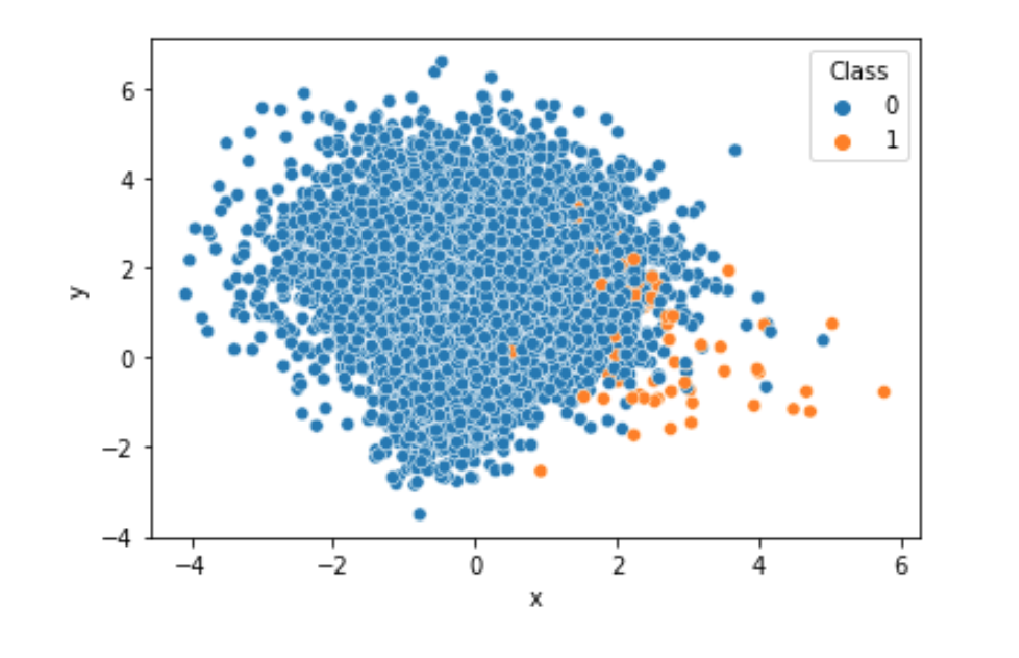
\includegraphics[scale=0.8]{image/data1.eps}
        \end{center}
    \end{figure*}
\end{center}

\subsection{German Credit Dataset}

The German Credit Dataset was downloaded from the UCI Machine Learning Repository, a web site that maintains many real datasets\cite{German}. 

The data set contains 1000 entries with 20 prepared category/symbol attributes
In this data set, each entry represents a person who receives credit from a bank. Each person is classified as a good or bad credit risk according to a set of attributes. We estimate it.
The data set is skewed with 700 out of 1000 entries for good credit risk.


\subsection{Haberman's Survival Data Set}

Haberman's Survival Data Set was similarly downloaded from the UCI Machine Learning Repository\cite{Haberman}.

The dataset contains case studies of survival of patients undergoing surgery for breast cancer conducted at the Billings Hospital of the University of Chicago between 1958 and 1970.
It has 306 data counts and three feature sets.
Estimate whether the patient died within 5 years.
It is a biased data set with 225 data that died within 5 years compared to 81 data that did not.

\subsection{Census-Income (KDD) Data Set}

The Census-Income (KDD) Data Set was similarly downloaded from the UCI Machine Learning Repository\cite{Census}.
This dataset contains weighted census data drawn from the 1994 and 1995 Current Population Surveys conducted by the U.S. Census Bureau. The data includes 41 demographic and employment related variables.
All categorical variables can be transformed into a Sparse One-Hot vector.
What we estimate is whether the income is greater than 50K or not.
We have a very large number of data, 32561, and the data is biased with 24720 being less than 50K.

\subsection{Blood Transfusion Service Center Data Set}

The Blood Transfusion Service Center Data Set was similarly downloaded from the UCI Machine Learning Repository\cite{Blood}.

This dataset contains data obtained from a blood transfusion service center located in Hsin Chu, Taiwan.
The center gives its blood transfusion service bus to one of the universities in Hsin Chu and collects donated blood about every three months. To build the marketing model which is a modified version of RFM, we randomly selected 748 donors from the donor database. For these 748 donor data, four variables were included. These are used to estimate whether a given donor has donated blood or not.

The data set is skewed, with 178 people who have donated blood compared to 570 who have not done so.
\clearpage


\section{Methods}
\subsection{SMOTE}

SMOTE is one method of random oversampling that increases the number of minority cases by randomly replicating the minority cases\cite{SMOTE}.

Below are the biased datasets.
Blue is the minority data set and orange is the majority data set.This can be seen in Fig. 2.2.

\begin{center}
    \begin{figure*}[ht]
        \caption{SMOTE: Before Oversampling.}
        \label{tab:team-rating-features}
        \begin{center}
            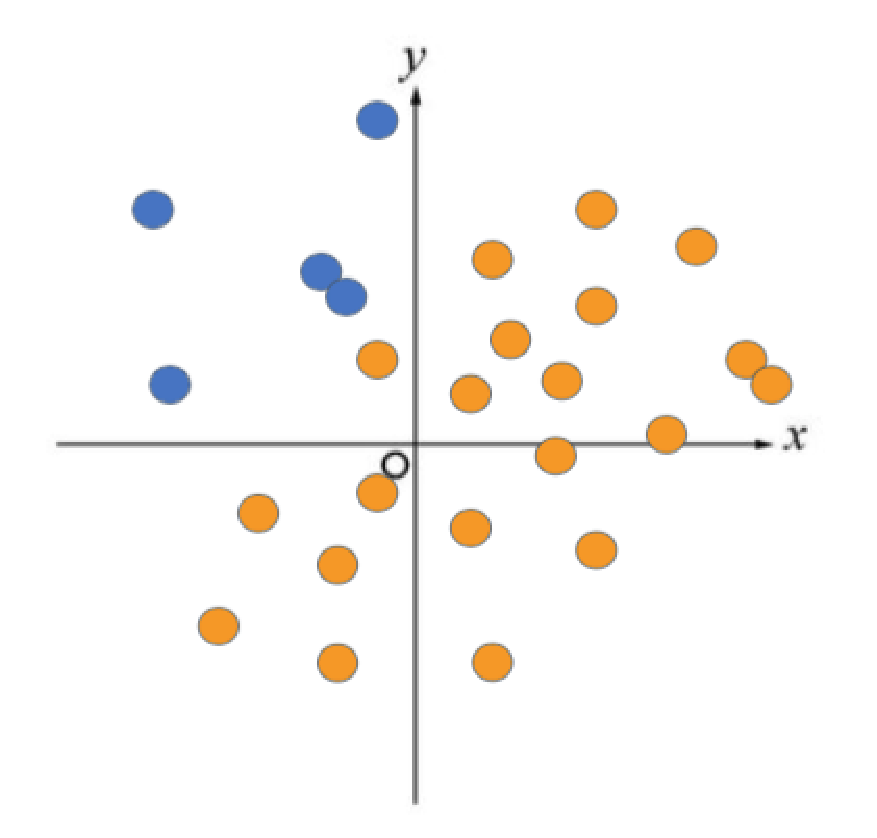
\includegraphics[scale=0.6]{image/smote1.eps}
        \end{center}
    \end{figure*}
\end{center}

\clearpage

Select one number group case. It's called $m_a$. This can be seen in Fig. 2.3.

\begin{center}
    \begin{figure*}[ht]
        \caption{SMOTE: Select a Case.}
        \label{tab:team-rating-features}
        \begin{center}
            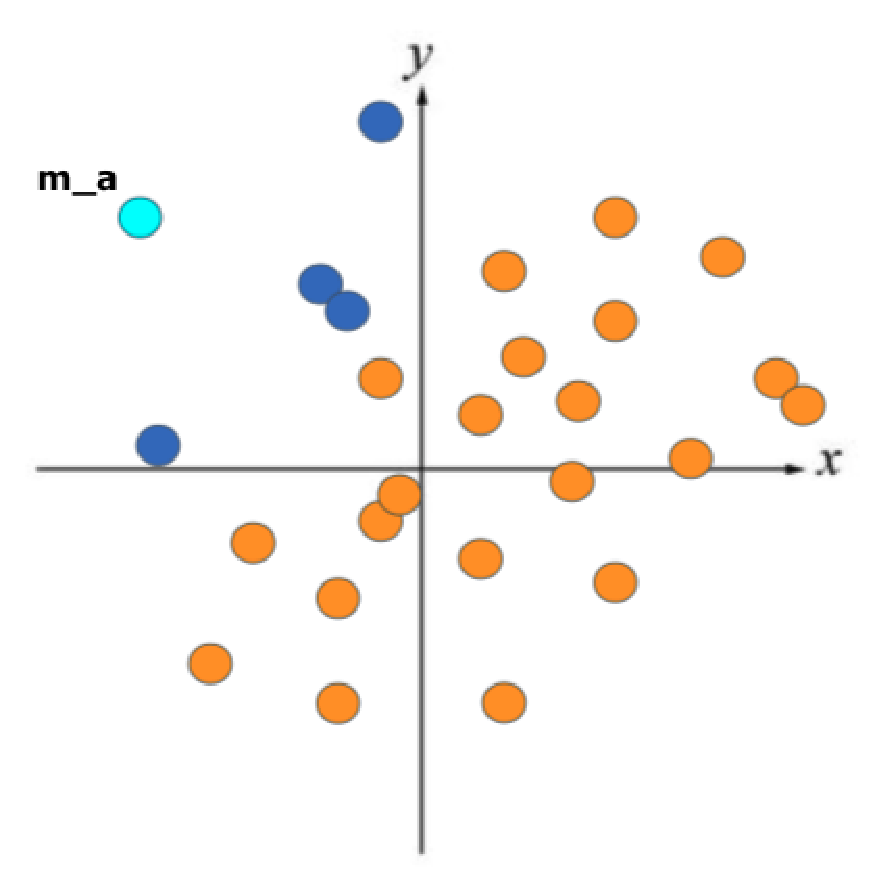
\includegraphics[scale=0.6]{image/smote2.eps}
        \end{center}
    \end{figure*}
\end{center}

\clearpage

Extract k data using the k-nearest neighbor method.
Calculate the degree of similarity between cases for a set of values of explanatory variables.
The similarity between vectors is calculated using the Euclidean distance

The j-th elements of $m_a$ and $m_i$ are written as $a_j$ and $i_j$, respectively.
$$
dis(m_a, m_i) = \Sigma_j(a_j - i_j)^2
$$
The figure below shows the k nearest neighbors painted in green. Figs2.4

\begin{center}
    \begin{figure*}[ht]
        \caption{SMOTE: Shows k nearest neighbor.}
        \label{tab:team-rating-features}
        \begin{center}
            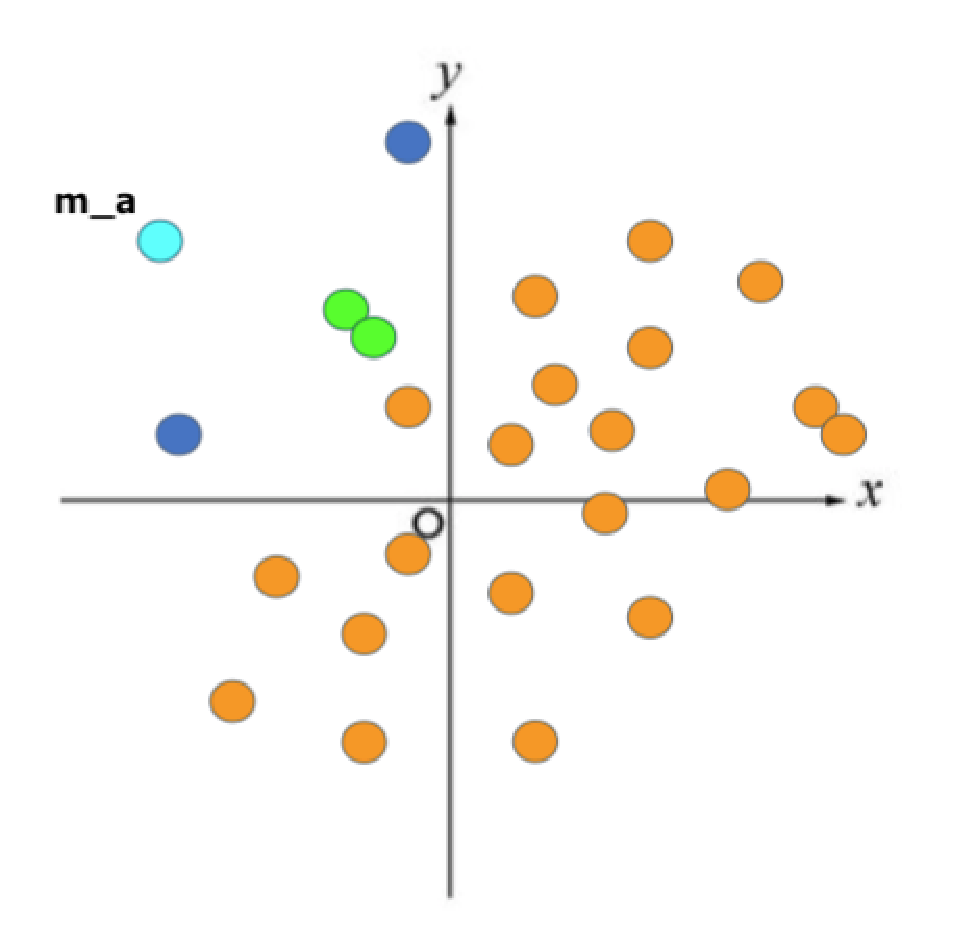
\includegraphics[scale=0.6]{image/smote3.eps}
        \end{center}
    \end{figure*}
\end{center}

\clearpage

Randomly select one of the k nearest neighbors.
In other words, pick one of the data that is colored green. Randomly.
I painted the selected one yellow.Figs2.5

\begin{center}
    \begin{figure*}[ht]
        \caption{SMOTE: Choose One Case from k nearest neighbors.}
        \label{tab:team-rating-features}
        \begin{center}
            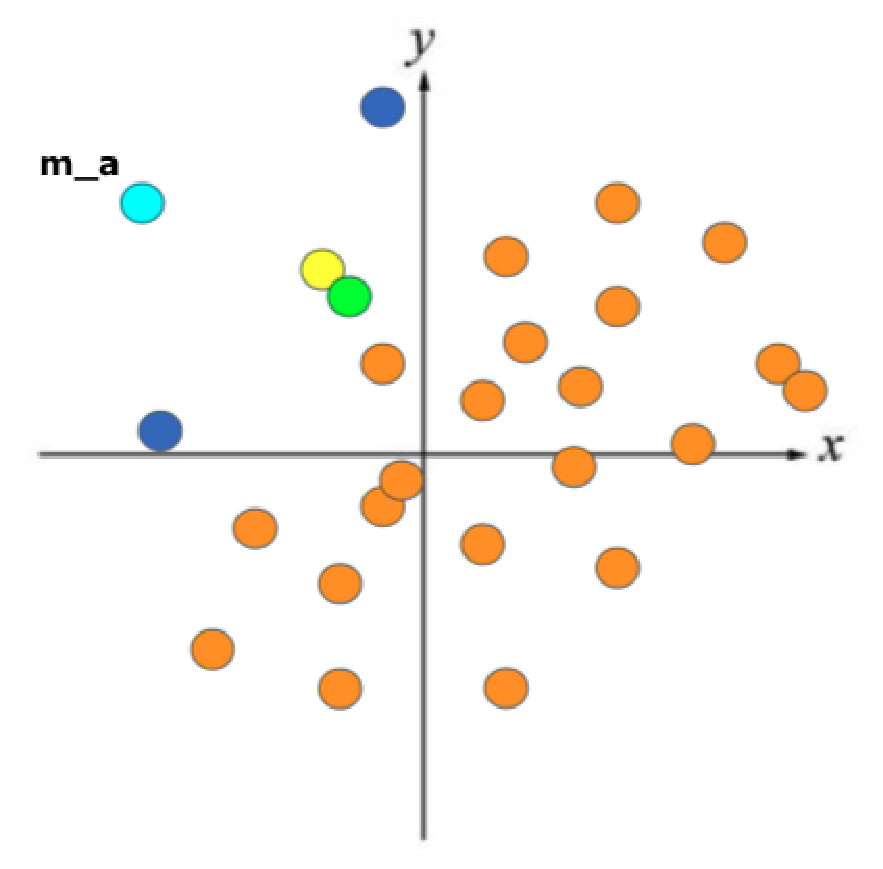
\includegraphics[scale=0.6]{image/smote4.eps}
        \end{center}
    \end{figure*}
\end{center}

\clearpage
Connect the first data you selected with the data you just selected with a straight line. Figs2.6.

\begin{center}
    \begin{figure*}[ht]
        \caption{SMOTE: Increase the number of new data in a linear fashion.}
        \label{tab:team-rating-features}
        \begin{center}
            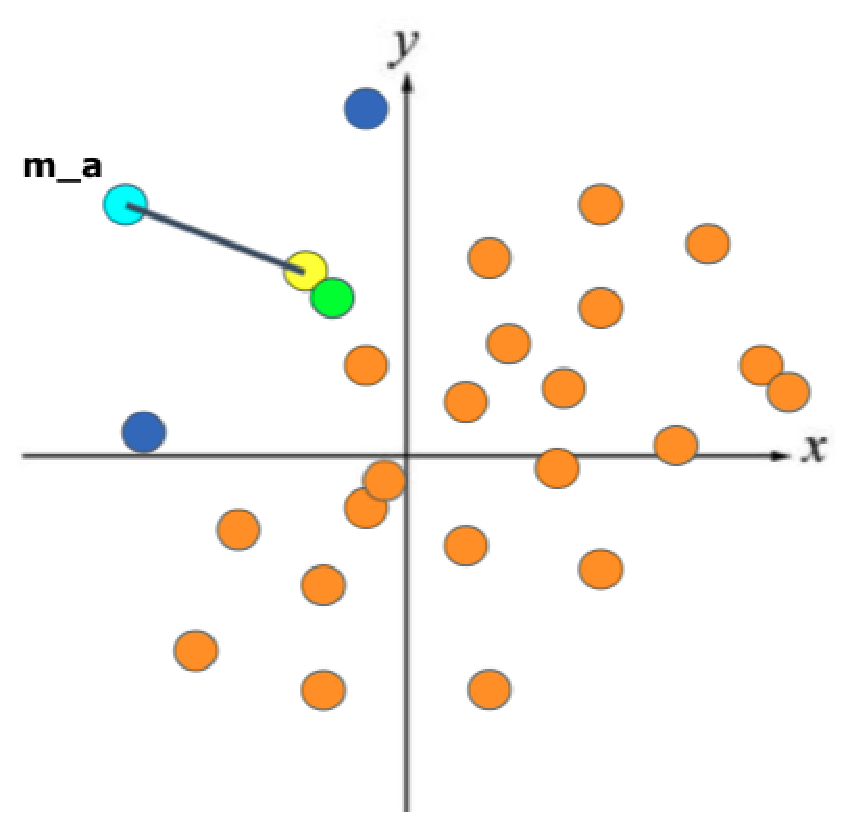
\includegraphics[scale=0.6]{image/smote5.eps}
        \end{center}
    \end{figure*}
\end{center}

It then generates some new data on that line.
This is the data that is generated by oversampling.
The position of the data on the line is completely random.

\clearpage
\subsection{Tomek-links}

One method of undersampling, which removes noisy samples, is to reduce the majority of the data set from a combination called Tomek Links\cite{TomekLinks}.

The algorithm is described below.
Below is a biased data set.
Blue is the minority data set and orange is the majority data set.

\begin{center}
    \begin{figure*}[ht]
        \caption{TOMEK-LINKS: Before undersampling dataset.}
        \label{tab:team-rating-features}
        \begin{center}
            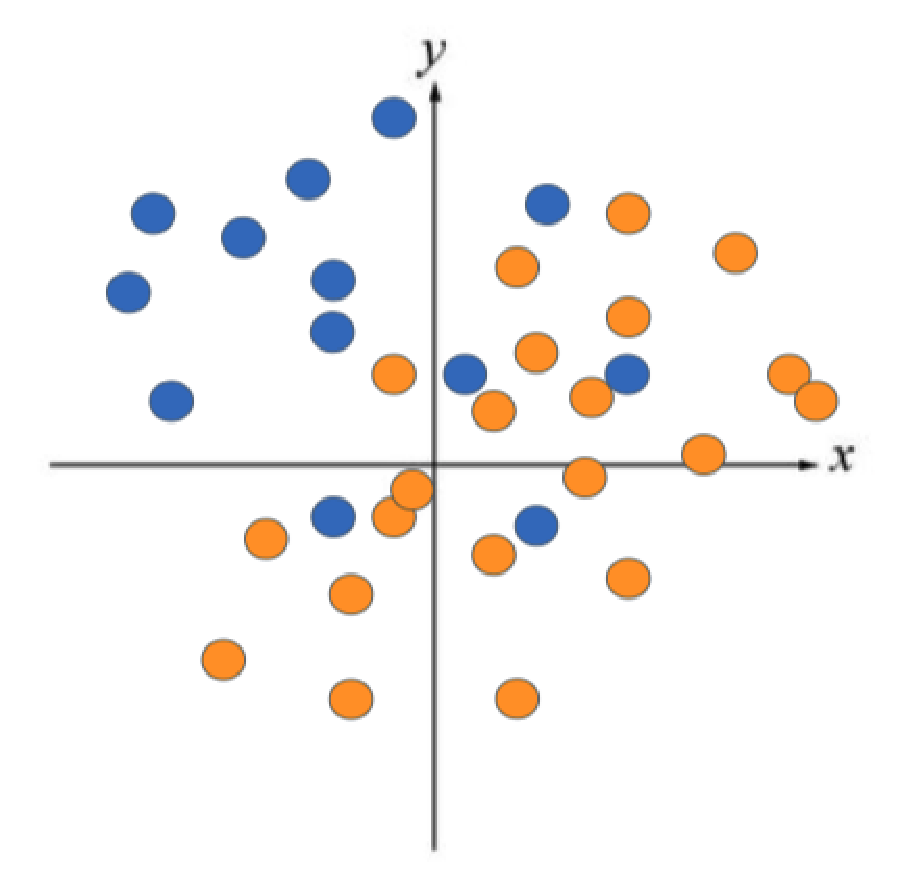
\includegraphics[scale=0.6]{image/tomek1.eps}
        \end{center}
    \end{figure*}
\end{center}

\clearpage

Tomek links are pairs of $x$ and $y$ such that there is no case $z$ in the dataset that satisfies $\delta(x, z) < \delta(x, y)$ or $\delta(y, z) < \delta(y, x)$.
However, we define $\delta(x, y)$ to be the distance between the minority case $x$ and the majority case $y$.

\begin{center}
    \begin{figure*}[ht]
        \caption{TOMEK-LINKS: Show the tomek-links.}
        \label{tab:team-rating-features}
        \begin{center}
            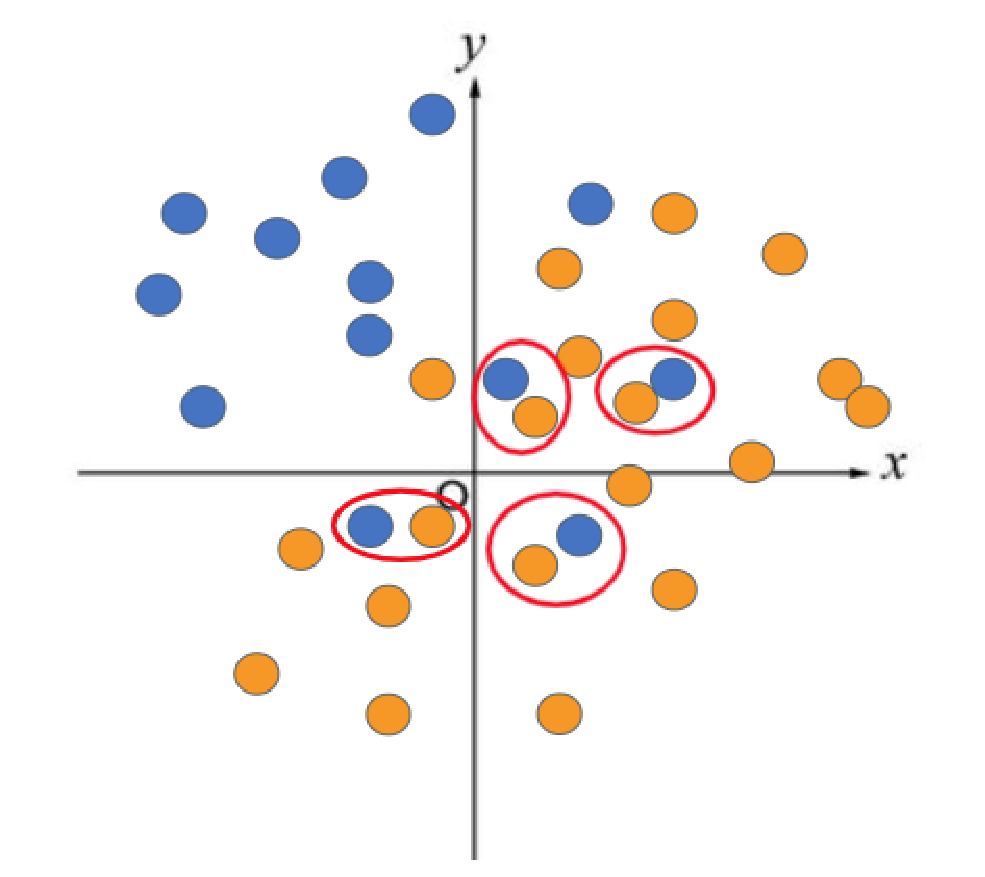
\includegraphics[scale=0.6]{image/tomek2.eps}
        \end{center}
    \end{figure*}
\end{center}

\clearpage

Delete the majority of data from these tomek links.

\begin{center}
    \begin{figure*}[ht]
        \caption{TOMEK-LINKS: Deleted tomek-links.}
        \label{tab:team-rating-features}
        \begin{center}
            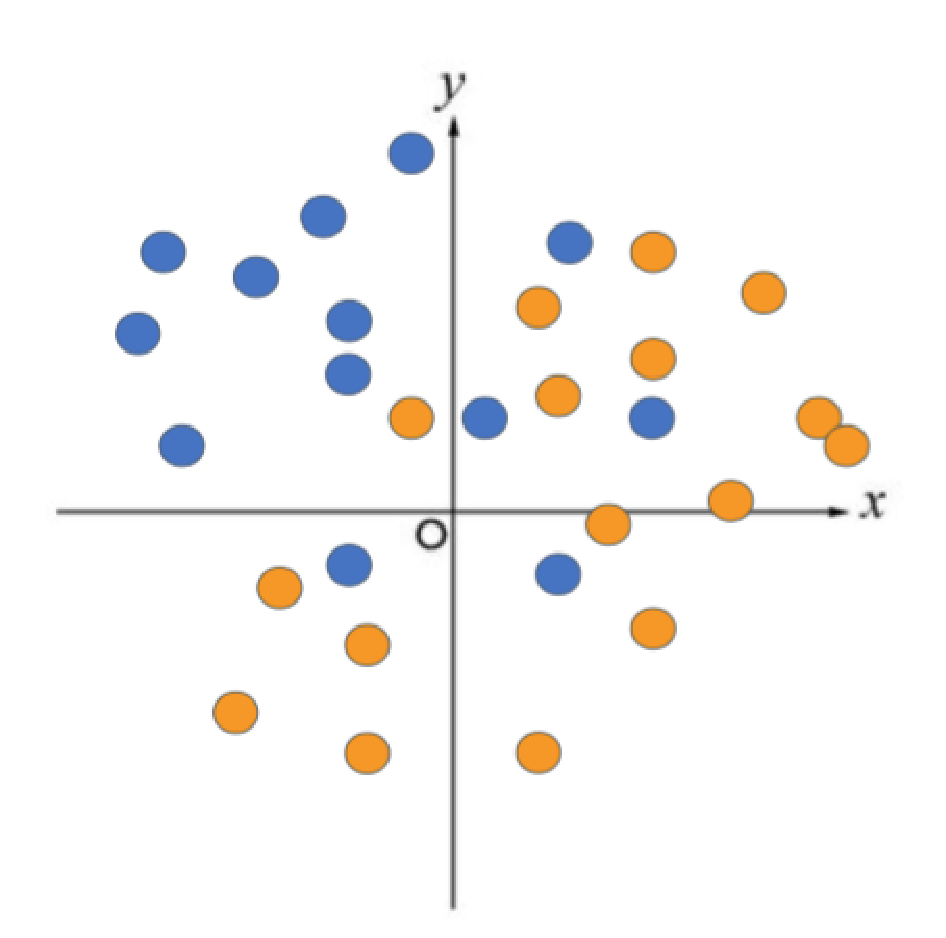
\includegraphics[scale=0.6]{image/tomek3.eps}
        \end{center}
    \end{figure*}
\end{center}

This process is repeated until there are no more two samples that are nearest neighbors of each other.
It prevents the majority from inferring that the training data has too much majority data, even if it has the characteristics of minority data.

\clearpage

\subsection{SMOTE + Tomek Combine}
In SMOTE + Tomek Combine, SMOTE and Tomek links are combined and over- and under-sampled.

\subsection{MySMOTE}

MySMOTE is an improved version of SMOTE.

Using a traditional SMOTE produces a linear data set.
In other words, linear data set is a straight line of data set
The boundaries between each class become blurred.
So, instead of sampling data on a straight line, I add noise and sampling data collectively.
The following is a description of the algorithm used by MySMOTE to perform oversampling.

\begin{center}
    \begin{figure*}[ht]
        \caption{MYSMOTE: How to calculate the noise.}
        \label{tab:team-rating-features}
        \begin{center}
            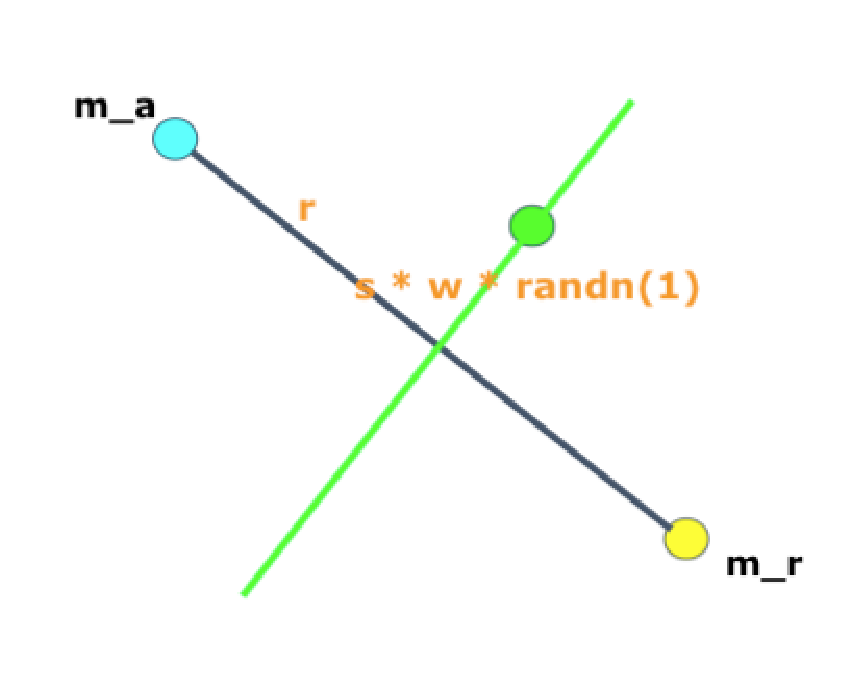
\includegraphics[scale=0.6]{image/mysmote1.eps}
        \end{center}
    \end{figure*}
\end{center}

Here is an explanation of the above variables.\\
$r$: This is a random value from $0$ to $1$ chosen uniformly.
This is the value used to determine the position of the new point generated between $m_a$ and $m_r$.
Noise is added to the point such that $m_a:m_r=r:1-r$, which is the new point.\\
$s$: Hyperparameter to determine how much noise to make.
The larger the value of $s$, the larger the noise will be.
The value range of $s$ is above 0.\\
$w$: This is the value of the variance of the explanatory variables.\\
I introduced it for the purpose of normalizing the magnitude of the noise to the explanatory variables.\\
$randn(1)$: randn outputs a random number with standard normal distribution.
The standard normal distribution is a Gaussian distribution with mean 0 and standard deviation 1.
This will randomly determine the size of the noise to be added.\\


Determine $m_a$ and $m_r$ as in SMOTE, and find the interior point such that $m_a:m_r=r:1-r$.
Up to this point, it is the same as SMOTE.
Then, the vector that is $s \times w \times randn(1)$ is called $\bm{v}$.
This $\bm{v}$ is noise.
Add $\bm{v}$ to the vector from the origin to its interior point.
In this way, we can now oversample not only the straight line connecting $m_a$ and $m_r$, but also the surrounding area.
By doing so, we aim to create a model that can determine the minority class for cases near the line connecting $m_a$ and $m_r$.

\section{What kind of model to experiment?}
As explained in the previous section, I train on a biased data set with some data preprocessing such as oversampling or undersampling.
I use scikit-learn to ensure that the learning is equal under all conditions. Decision Tree is used as the machine learning algorithm.
It is easy to think that decision trees are confusing when learning imbalanced data. This is because it removes branches that are considered to be too specialized and labels the new leaf nodes with the dominant class.
It becomes more likely that the majority class will become the dominant class of these leaf nodes, and it will not be able to capture the characteristics of the minority class.
To see if such a problem can be solved using oversampling or undersampling, a decision tree is used.
The details of the actual model used are as follows.

\begin{lstlisting}[caption=DecisionTreeClassifier,label=DecisionTreeClassifier]
sklearn.tree.DecisionTreeClassifier(*,
     criterion='gini',
     splitter='best',
     max_depth=3,
     min_samples_split=2,
     min_samples_leaf=1,
     min_weight_fraction_leaf=0.0,
     max_features=None,
     random_state=None,
     max_leaf_nodes=None,
     min_impurity_decrease=0.0,
     min_impurity_split=None,
     class_weight=None,
     ccp_alpha=0.0
)
\end{lstlisting}


\section{How to evaluate the model?}
A very commonly used evaluation metric for machine learning models is accuracy.
An index to determine how well the answer matches the overall prediction result. See below for the calculation formula.
$$
Accuracy = \frac{TP + TN}{TP + TN + FP + FN}
$$
And, $TP$ is the number of True Positive, $TN$ is the number of True Negative, $FP$ is the number of False Positive, and $FN$ is the number of False Negative cases. This section uses such an abbreviation.

Accuracy is an unreliable metric in imbalanced data.
This is because they can simply produce a high score.
For example, consfider a data set where 80 percent of the data is in the majority class and 20 percent in the minority class. If we have a model that labels all the data as majority class, the accuracy of the model will be 0.8.
This number is high, but it does not mean that this model is meaningless.
As the class distribution changes, so do these metrics, even if the performance of the underlying classifier does not change.
So it would be more interesting to use a performance metric that separates out the errors (or hits) that occur in each class.
In terms of these factors, I will use the AUC index\cite{ROC}.

The term AUC comes from Area Under the Curve.
The curve is the ROC curve, and the area of the lower right part is called the AUC.
And the ROC curve is a line graph in which the points corresponding to the vertical axis: true positive rate, and the horizontal axis: false positive rate, are plotted and connected for every $p$, assuming that "the estimated probability is greater than or equal to $p$ is considered positive.
Two more indicators will be introduced.
These are Precision and Recall.

Recall is a measure that refers to how many minority class cases were predicted without any oversights.
In other words, it is the percentage of minority class cases that are correctly determined to be minority class cases.
This is an important indicator when you want to ensure the success of your minority class inference.
$$
Recall = \frac{TP}{TP + FN}
$$
Precision is the percentage of patients predicted to be in the minority class that are really in the minority class.
In other words, it is the accuracy of the prediction of the minority class.
This indicator tends to decrease when you try to increase the Recall.
$$
Precision = \frac{TP}{TP + FP}
$$
